\documentclass[12pt,a4paper]{report}
% For pdfLaTeX encoding
\usepackage[utf8]{inputenc}
\usepackage[T1]{fontenc}

\usepackage[french]{babel} 
\usepackage{csquotes}
\usepackage{a4wide}
\usepackage{graphicx}
\usepackage{placeins}
\usepackage{tikz}
\usetikzlibrary{chains}
\usetikzlibrary{chains,arrows.meta,positioning,decorations.pathreplacing}
% Custom arrow tip for open circle
\tikzset{
  open arrow/.style = {-{Circle[open]}, shorten <=1pt, shorten >=1pt}
}

\usepackage{pgfplots}
%pour la mise en page des tableaux
\usepackage{array}
\usepackage{tabularx}
\usepackage[table,xcdraw]{xcolor}
\usepackage{wrapfig}
\usepackage{subcaption}
\usepackage{color, colortbl}
\definecolor{Gray}{gray}{0.9}
\definecolor{LightCyan}{rgb}{0.88,1,1}
\usepackage{longtable}
\usepackage{float}
\usepackage{xcolor}
\usepackage{array} % for extrarowheight
\usepackage{lscape}
\usepackage{afterpage}
\usepackage{rotating}
\usepackage[nottoc,notlof,notlot]{tocbibind}
\usepackage{tocloft}
\usepackage{pdfpages}
\graphicspath{../images/}
\newlength\figureheight
\newlength\figurewidth
\usepackage{ifthen}
\usepackage{ifpdf}
\ifpdf
\usepackage[pdftex]{hyperref}
\else
\usepackage{hyperref}
\fi
\usepackage{color}
\hypersetup{%
colorlinks=true,
linkcolor=black,
citecolor=black,
urlcolor=blue}
% \urlstyle{same}
\usepackage[top=2.5cm,bottom=2.5cm,right=2.5cm,left=2.5cm]{geometry}
\usepackage{changepage}

\usepackage{tabularx}
    \newcolumntype{L}{>{\raggedright\arraybackslash}X}
\usepackage{longtable}

\usepackage{xltabular}
\renewcommand{\tablename}{Tableau}
\renewcommand{\figurename}{Figure}

\raggedbottom

%pour les références bibliographiques
\usepackage[style=numeric,sorting=nyt,backend=biber]{biblatex}
\addbibresource{bibliography/references.bib}



% \DefineBibliographyStrings{french}{
%   urlseen = {consulté en}
% }
% \DeclareFieldFormat{urldate}{\mkdate#1}

% \AtEveryBibitem{
%   \ifentrytype{misc}{
%     \clearlist{author}
%     \clearfield{title}
%     \clearfield{note}
%     \clearfield{year}
%     \clearfield{month}
%     \clearfield{day}
%     \clearfield{howpublished}
%     \renewbibmacro*{begentry}{} % supprime l'année avant le lien
%     \renewbibmacro*{finentry}{\par}
%     \renewbibmacro*{url+urldate}{%
%       \printfield{url}%
%       \iffieldundef{urldate}
%         {}
%         { (consulté en \printurldate)}
%     }
%   }{
%     \clearfield{url}
%     \clearfield{urlyear}
%   }
% }

% Only once
\usepackage{xurl}
\usepackage[colorlinks=true,linkcolor=black,citecolor=black,urlcolor=blue,breaklinks]{hyperref}


% pour les algorithmes
\usepackage[linesnumbered,ruled,vlined]{algorithm2e}
\SetKwInput{KwInput}{Input}
\DontPrintSemicolon





\setlength\arrayrulewidth{1pt}
\renewcommand{\baselinestretch}{1.05}
\usepackage{fancyhdr}
\pagestyle{fancy}
\fancyhf{}
\lhead{\bfseries\nouppercase{\leftmark}}
\rfoot{\bfseries\thepage}
\setlength{\headheight}{14.5pt}

\let\headruleORIG\headrule

\renewcommand{\headrule}{\color{black} \headruleORIG}
\renewcommand{\headrulewidth}{1.0pt}
\usepackage{colortbl}
\arrayrulecolor{black}

\fancypagestyle{plain}{
  \fancyhead{}
  \fancyfoot[R]{\bfseries\thepage}
  \renewcommand{\headrulewidth}{0pt}
}



\makeatletter
\def\@textbottom{\vskip \z@ \@plus 1pt}
\let\@texttop\relax
\makeatother

\makeatletter
\def\cleardoublepage{\clearpage\if@twoside \ifodd\c@page\else%
  \hbox{}%
  \thispagestyle{empty}%
  \newpage%
  \if@twocolumn\hbox{}\newpage\fi\fi\fi}
\makeatother

\usepackage{amsthm}
\usepackage{array}
\usepackage{bm}
\usepackage{multirow}
\usepackage[footnote]{acronym}

\usepackage{amssymb,amsmath,bbm,mathtools}
\DeclareMathOperator*{\argmin}{arg\,min}

\usepackage[bottom]{footmisc}


% — permettre la numérotation jusqu’au 4ᵉ niveau (paragraph)
\setcounter{secnumdepth}{4}
% — dans la table des matières, ne pas dépasser le 2ᵉ niveau (subsection)
\setcounter{tocdepth}{2}

% — on va “recycler” \paragraph comme sous-sous-sous-section numérotée
\usepackage{titlesec}

% définir le format du numéro : section.subsection.subsubsection.paragraph
\renewcommand\theparagraph{%
  \thesection.\thesubsection.\thesubsubsection.\arabic{paragraph}%
}

% styler \paragraph pour qu’il ressemble à une vraie section
\titleformat{\paragraph}[hang]
  {\normalfont\normalsize\bfseries}   % police
  {\theparagraph}                     % label
  {1em}                               % espace label–titre
  {}                                  % code avant le titre

% ajuster les espacements verticaux de \paragraph
\titlespacing*{\paragraph}
  {0pt}                               % retrait gauche
  {3.25ex plus 1ex minus .2ex}        % avant
  {1em}                               % après

\newtheoremstyle{break}
  {11pt}{11pt}%
  {\itshape}{}%
  {\bfseries}{}%
  {\newline}{}%
\theoremstyle{break}

%\theoremstyle{definition}
\newtheorem{definition}{Définition}[chapter]

%\theoremstyle{definition}
\newtheorem{theoreme}{Théorème}[chapter]

%\theoremstyle{remark}
\newtheorem{remarque}{Remarque}[chapter]

%\theoremstyle{plain}
\newtheorem{propriete}{Propriété}[chapter]
\newtheorem{exemple}{Exemple}[chapter]

%table break line

\usepackage{makecell}

\renewcommand\theadalign{bl}
\renewcommand\theadfont{\bfseries}
\renewcommand\cellalign{bl}
\renewcommand\cellgape{\Gape[2pt]}

\parskip=5pt
%\sloppy
 %%%%********************************************************************
\definecolor{quotemark}{gray}{0.7}
\makeatletter
\def\fquote{%
    \@ifnextchar[{\fquote@i}{\fquote@i[]}%]
           }%
\def\fquote@i[#1]{%
    \def\tempa{#1}%
    \@ifnextchar[{\fquote@ii}{\fquote@ii[]}%]
                 }%
\def\fquote@ii[#1]{%
    \def\tempb{#1}%
    \@ifnextchar[{\fquote@iii}{\fquote@iii[]}%]
                      }%
\def\fquote@iii[#1]{%
    \def\tempc{#1}%
    \vspace{1em}%
    \noindent%
    \begin{list}{}{%
         \setlength{\leftmargin}{0.1\textwidth}%
         \setlength{\rightmargin}{0.1\textwidth}%
                  }%
         \item[]%
         \begin{picture}(0,0)%
         \put(-15,-5){\makebox(0,0){\scalebox{3}{\textcolor{quotemark}{``}}}}%
         \end{picture}%
         \begingroup\itshape}%
 %%%%********************************************************************
 \def\endfquote{%
 \endgroup\par%
 \makebox[0pt][l]{%
 \hspace{0.8\textwidth}%
 \begin{picture}(0,0)(0,0)%
 \put(15,15){\makebox(0,0){%
 \scalebox{3}{\color{quotemark}''}}}%
 \end{picture}}%
 \ifx\tempa\empty%
 \else%
    \ifx\tempc\empty%
       \hfill\rule{100pt}{0.5pt}\\\mbox{}\hfill\tempa,\ \emph{\tempb}%
   \else%
       \hfill\rule{100pt}{0.5pt}\\\mbox{}\hfill\tempa,\ \emph{\tempb},\ \tempc%
   \fi\fi\par%
   \vspace{0.5em}%
 \end{list}%
 }%
 \makeatother
 %%%%********************************************************************
 
 
 \usepackage{afterpage}

\newcommand\blankpage{%
    \null
    \thispagestyle{empty}%
    \addtocounter{page}{-1}%
    \newpage}
    
\renewcommand{\listalgorithmcfname}{Liste des algorithmes}

\newcommand{\mychapter}[2]{
    
    \chapter*{#2}
    \addcontentsline{toc}{chapter}{#2}
}

\usepackage[page,toc,titletoc,title]{appendix}

\addto\captionsfrench{%
  \renewcommand\appendixname{Annexe}
  \renewcommand\appendixpagename{Annexes}
  \renewcommand{\appendixtocname}{Annexes}
}
\usepackage{etoolbox}
\appto\appendix{\addtocontents{toc}{\protect\setcounter{tocdepth}{0}}}

% reinstate the correct level for list of tables and figures and algorithms
\appto\listoffigures{\addtocontents{lof}{\protect\setcounter{tocdepth}{1}}}
\appto\listoftables{\addtocontents{lot}{\protect\setcounter{tocdepth}{1}}}
\appto\listofalgorithms{\addtocontents{loa}{\protect\setcounter{tocdepth}{1}}}



\usepackage{graphicx}     % pour \includegraphics
\usepackage{booktabs}     % \toprule, \midrule, \bottomrule
\usepackage{subcaption}   % environnement subfigure
\usepackage{siunitx}      % \num, \SI, \percent
\sisetup{detect-all}
\usepackage{pifont}       % symboles ✓ et ✗
\newcommand{\cmark}{\ding{51}}   % ✓
\newcommand{\xmark}{\ding{55}}   % ✗
\DeclareUnicodeCharacter{2009}{\,}



\raggedbottom
\usepackage[french]{babel} 
\usepackage{mdframed}

\begin{document}

\thispagestyle{empty}

% En-tête avec les logos - taille optimisée
\noindent
\hfill%
\begin{center}
\begin{minipage}{0.7\textwidth}
  \raggedleft
  
\includegraphics[width=10cm]{images/LogoIbnZohr.png}
\end{minipage}
\end{center}
\vspace{1.8cm}

% Code de formation
\begin{flushright}
 \large ENSA5/FID/2025-2026
\end{flushright}

\vspace{1cm}

% Titre principal
\begin{center}
  \textbf{\Large Rapport de Projet Valorisation de produits dérivés et
couverture}
\end{center}


\vspace{1cm}

% Spécialité
\begin{center}
  \large Spécialité : \textbf{Finance et Ingénierie Décisionnelle}
\end{center}

\vspace{1cm}

% Thème - TITRE AGRANDI
\begin{center}
   \large Intitulé :
  
  \vspace{0.4cm}
  {\LARGE\bfseries Valorisation d'Options Américaines :\\
  \vspace{0.4cm}
  Frontières d'Exercice Optimal sous Régimes Markoviens}
\end{center}
\vspace{1.8cm}
\begin{center}    
    \large Présenté par : \\
    \textbf{Achraf HAJJI} 
    \vspace{1cm}
    
     \large Sous la direction de : \\
     Pr. Brahim EL ASRI 
    \vspace{1cm}
    
  \textbf{ Année universitaire 2025-2026} 
\end{center}
\end{titlepage}

% Remerciements
\chapter*{Remerciements}
\addcontentsline{toc}{chapter}{Remerciements}

Je souhaite exprimer ma profonde gratitude à l'ensemble de mes professeurs pour les efforts qu'ils ont déployés tout au long de ma formation. Leur engagement constant, la richesse de leur enseignement et leur rigueur intellectuelle ont constitué les piliers de mon parcours académique.

Je tiens à remercier particulièrement le Professeur Brahim EL ASRI pour sa direction attentive, ses conseils précieux et sa disponibilité durant l'élaboration de ce mémoire. Son expertise dans le domaine de la finance quantitative et ses orientations judicieuses m'ont permis de mener à bien ce projet.

Mes remerciements vont également à toutes les personnes qui, de près ou de loin, ont contribué au bon déroulement de ce travail. Bien que je ne puisse les citer individuellement, qu'elles trouvent ici l'expression de ma reconnaissance sincère.

Enfin, je voudrais témoigner ma gratitude envers ma famille pour son soutien inconditionnel et ses encouragements constants tout au long de mon parcours universitaire.

\clearpage

% Liste des figures
\listoffigures
\clearpage

% Liste des abréviations
\chapter*{Liste des abréviations}
\addcontentsline{toc}{chapter}{Liste des abréviations}

\begin{tabular}{p{0.15\textwidth} p{0.8\textwidth}}
T & Echéance d'une option \\
AOA & Absence d'Opportunité d'Arbitrage \\
u & Facteur de hausse d'un actif risqué \\
d & Facteur de baisse d'un actif risqué \\
r & Taux sans risque \\
$\sigma$ & Volatilité de l'actif risqué \\
C & Produit dérivé \\
x & Capital initial \\
t & Variable temporelle \\
$S_0$ & Cours de l'actif risqué à $t=0$ \\
$W_t$ & Le mouvement brownien unidimensionnel \\
K & Le strike d'une option \\
CRR & Cox-Rubistein-Ross \\
N & La fonction de répartition de la loi centrée réduite \\
\end{tabular}

\clearpage

% Table des matières
\tableofcontents
\clearpage

% Introduction
\chapter*{Introduction}
\addcontentsline{toc}{chapter}{Introduction}

Ce travail porte sur la valorisation des options financières, avec une attention particulière à l'amélioration du modèle binomial par l'ajout de régimes de marché.
\end{mdframed}

\vspace{0.5cm}

La valorisation des produits dérivés représente un enjeu majeur pour les marchés financiers. Ces instruments, particulièrement les options, permettent aux investisseurs de se couvrir contre les risques ou de spéculer sur l'évolution future des prix. Leur évaluation précise est donc essentielle pour garantir l'efficacité et l'équité des transactions.

\vspace{0.3cm}

Le modèle binomial, développé par Cox, Ross et Rubinstein en 1979, offre une méthode simple et intuitive pour valoriser les options. Dans ce cadre, le prix de l'actif sous-jacent peut seulement monter ou descendre à chaque période, créant un arbre de possibilités. Cette approche en temps discret permet de comprendre facilement les mécanismes fondamentaux de la valorisation et s'applique aussi bien aux options européennes qu'américaines.

\vspace{0.3cm}

Parallèlement, le modèle de Black \& Scholes, formulé en 1973, propose une solution analytique pour les options européennes en temps continu. On peut démontrer que le modèle binomial converge vers celui de Black \& Scholes lorsque le nombre de périodes tend vers l'infini, établissant ainsi un lien important entre ces deux approches.

\vspace{0.3cm}

Cependant, ces modèles classiques reposent sur une hypothèse restrictive: la volatilité du marché reste constante. Cette simplification ne correspond pas à la réalité des marchés financiers qui alternent entre des périodes calmes et des périodes agitées. Le phénomène bien connu des "smiles de volatilité" témoigne de cette inadéquation.

\vspace{0.3cm}

Pour répondre à cette limitation, nous proposons d'enrichir le modèle binomial en y ajoutant des régimes de marché gérés par des chaînes de Markov. Cette extension permet à la volatilité de changer selon l'état du marché (calme ou agité), tout en conservant la simplicité conceptuelle du modèle original. Notre approche s'avère particulièrement utile pour les options américaines, dont la décision d'exercice dépend fortement des conditions de marché.

\vspace{0.3cm}

Notre étude se divise en deux parties principales. D'abord, nous présentons les bases théoriques des modèles binomiaux et de Black \& Scholes, avant d'introduire notre extension avec régimes de marché. Ensuite, nous développons une application Python qui permet de comparer ces différents modèles et de visualiser l'impact des changements de régime sur les prix des options et les frontières d'exercice optimal.



% Corps du document
\chapter{Partie Théorique}
\section{Espace et hypothèses de travail}

Cette section établit le cadre mathématique rigoureux dans lequel nous développerons nos modèles de valorisation d'options. Nous commencerons par la modélisation probabiliste du marché dans sa forme la plus élémentaire, puis nous préciserons les hypothèses économiques qui sous-tendent notre approche.

\subsection{Modélisation probabiliste du marché}

Considérons un marché à deux actifs et deux dates : $t = 0$ et $t = 1$.

\begin{itemize}
    \item \textbf{Un actif sans risque} qui vaut 1 en $t = 0$ et vaut $R = (1 + r)$ en $t = 1$, représentant l'argent placé à la banque au taux $r$ (dans une obligation). 
    $$1 \rightarrow R = 1 + r$$
    
    \item \textbf{Un actif risqué $S$} de valeur $S_0$ en $t = 0$ et pouvant prendre deux valeurs différentes à l'instant 1 : une valeur haute $S_1^u = u \cdot S_0$ et une valeur basse $S_1^d = d \cdot S_0$ avec $u$ et $d$ deux constantes telles que $d < u$.
\end{itemize}

\begin{center}
\begin{tikzpicture}[scale=1.2]
    \node (start) at (0,0) {$S_0$};
    \node (up) at (2,1) {$uS_0$};
    \node (down) at (2,-1) {$dS_0$};
    \draw[->] (start) -- (up);
    \draw[->] (start) -- (down);
\end{tikzpicture}
\end{center}

La modélisation probabiliste du marché est la donnée de 3 objets : $\Omega$, $\mathcal{F}$ et $\mathbb{P}$.

\begin{itemize}
    \item $\Omega$ est l'ensemble des états du monde : 2 états possibles selon la valeur de l'actif risqué en $t = 1$, état "haut" $\omega_u$ ou "bas" $\omega_d$. $\Omega = \{\omega_u, \omega_d\}$
    
    \item $\mathbb{P}$ est la probabilité historique sur $\Omega$. $\mathbb{P}(\omega_u) = p$ et $\mathbb{P}(\omega_d) = 1 - p$. Le prix a une probabilité réelle $p$ de monter et $1 - p$ de descendre. Attention $p \in ]0, 1[$ car les 2 états du monde peuvent arriver.
    
    \item $\mathcal{F} = \{\mathcal{F}_0, \mathcal{F}_1\}$ est un couple de tribus représentant l'information globale disponible sur le marché aux instants $t = 0$ et $t = 1$.
    \begin{itemize}
        \item En $t = 0$, on ne dispose d'aucune information : $\mathcal{F}_0 = \{\emptyset, \Omega\}$.
        \item En $t = 1$, on sait si l'actif est monté ou descendu : $\mathcal{F}_1 = \mathcal{P}(\Omega) = \{\emptyset, \Omega, \{\omega_u\}, \{\omega_d\}\}$.
    \end{itemize}
\end{itemize}

\subsection{Extension aux régimes de marché}

Notre contribution consiste à enrichir ce cadre probabiliste en introduisant des régimes de marché. Dans cette approche étendue, nous considérons que le marché peut se trouver dans différents états ou régimes (par exemple, un régime calme ou un régime volatile), et que ces régimes influencent les paramètres du modèle, notamment la volatilité.


Formellement, nous introduisons un processus de Markov $(R_t)_{t \geq 0}$ à valeurs dans un ensemble fini d'états $\{0, 1, ..., K-1\}$, où chaque état représente un régime de marché. La probabilité de transition d'un régime à un autre est donnée par une matrice de transition $P = (p_{ij})$, où $p_{ij}$ représente la probabilité de passer du régime $i$ au régime $j$ dans la période suivante.


Dans ce cadre étendu, les paramètres du modèle binomial, notamment les facteurs de hausse et de baisse $u$ et $d$, dépendent du régime courant:

$$u(R_t) = e^{\sigma(R_t) \sqrt{\Delta t}}$$
$$d(R_t) = e^{-\sigma(R_t) \sqrt{\Delta t}}$$

où $\sigma(R_t)$ est la volatilité associée au régime $R_t$.

Cette extension permet de capturer les changements de dynamique du marché tout en conservant la structure binomiale fondamentale, offrant ainsi un modèle plus réaliste pour la valorisation des produits dérivés.

\begin{figure}[H]
\centering
\begin{tikzpicture}[scale=1]
    % Régime 0 (calme)
    \node[draw, circle] (r0) at (0,2) {$R_0=0$};
    \node (s00) at (0,0) {$S_0$};
    \node (s0u) at (2,1) {$u_0S_0$};
    \node (s0d) at (2,-1) {$d_0S_0$};
    \draw[->] (s00) -- (s0u);
    \draw[->] (s00) -- (s0d);
    
    % Régime 1 (volatil)
    \node[draw, circle] (r1) at (7.5,2) {$R_0=1$};
    \node (s10) at (7.5,0) {$S_0$};
    \node (s1u) at (9.5,1.5) {$u_1S_0$};
    \node (s1d) at (9.5,-1.5) {$d_1S_0$};
    \draw[->] (s10) -- (s1u);
    \draw[->] (s10) -- (s1d);
    
    % Transitions entre régimes (plus longues)
    \draw[->, bend left=20] (r0) to node[above] {$p_{01}$} (r1);
    \draw[->, bend left=20] (r1) to node[below] {$p_{10}$} (r0);
    \draw[->] (r0) to[loop above] node[above] {$p_{00}$} (r0);
    \draw[->] (r1) to[loop above] node[above] {$p_{11}$} (r1);
\end{tikzpicture}
\caption{Modèle binomial à deux régimes : régime calme (gauche) et régime volatil (droite)}
\label{fig:two_regime_model}
\end{figure}

\subsection{Hypothèses fondamentales}

Pour tous les modèles présentés dans ce travail, nous adoptons les hypothèses suivantes:

\begin{enumerate}
    \item \textbf{Absence d'opportunité d'arbitrage}: Il n'existe pas de stratégie permettant de réaliser un profit sans risque et sans capital initial.
    
    \item \textbf{Marché complet}: Tout actif contingent peut être répliqué par une combinaison appropriée des actifs disponibles.
    
    \item \textbf{Absence de frictions}: Les transactions s'effectuent sans coûts de transaction et les actifs sont parfaitement divisibles.
    
    \item \textbf{Taux d'intérêt constant}: Le taux d'intérêt sans risque $r$ reste constant sur toute la période considérée.
\end{enumerate}

Ces hypothèses, bien que simplificatrices, sont essentielles pour développer un cadre cohérent de valorisation.



\section{Modèle Binomial à une période}



Le modèle binomial à une période constitue le fondement conceptuel de notre approche. Il offre un cadre simple mais puissant pour comprendre les mécanismes de valorisation des produits dérivés.


Dans le modèle binomial à une période, nous distinguons deux instants $n=0$ et $n=1$. À l'instant $n=1$, nous supposons que soit le prix de l'actif risqué monte avec une probabilité $p$ ou il descend avec une probabilité $(1-p)$ comme sur la figure ci-dessous.

\begin{figure}[h]
\centering
\begin{tikzpicture}[scale=1.2]
    \node (start) at (0,0) {$S_0$};
    \node (up) at (2,1) {$uS_0$};
    \node (down) at (2,-1) {$dS_0$};
    \draw[->] (start) -- node[above] {$p$} (up);
    \draw[->] (start) -- node[below] {$1-p$} (down);
\end{tikzpicture}
\caption{Évolution du prix de l'actif sous-jacent dans le modèle binomial à une période}
\label{fig:one_period}
\end{figure}

De façon objective, à partir de ce modèle et d'un certain nombre d'inputs, nous aimerions déterminer le prix d'un produit dérivé à l'instant $n=0$ ainsi que le capital initial et la quantité d'actif risqué qui nous permettrait à l'instant $n=1$ d'avoir une rentabilité donnée.

Donc nous pouvons maintenant définir :
\begin{itemize}
    \item $\Omega = \{\omega_u, \omega_d\}$ donc il y'a deux états de la nature possible.
    \item $\mathcal{F} = \{\mathcal{F}_0, \mathcal{F}_1\}$ avec $\mathcal{F}_1 = \sigma(S_1)$
    \item $\mathbb{P}(\omega_u) = p$ et $\mathbb{P}(\omega_d) = 1 - p$
\end{itemize}

Cette représentation simple permet de modéliser l'incertitude fondamentale des marchés financiers : la possibilité que les prix montent ou baissent. Malgré sa simplicité apparente, ce modèle capture l'essence du comportement des actifs financiers et constitue la base sur laquelle nous construirons des modèles plus sophistiqués.

Dans les sections suivantes, nous allons explorer comment construire une stratégie de portefeuille qui permet de répliquer un produit dérivé, puis comment déterminer son prix juste en utilisant le principe d'absence d'opportunité d'arbitrage.




  \subsection{Stratégie de portefeuille simple}

Nous travaillons dans un marché complet donc nous pouvons déterminer une stratégie $(x, \Delta)$ qui duplique $C$ un produit dérivé.

En effet, à l'instant $n=1$ nous avons :
\begin{align*}
C_1^u &= \Delta S_1^u + (x - \Delta S_0)R = xR + (u-R)\Delta S_0 \\
C_1^d &= \Delta S_1^d + (x - \Delta S_0)R = xR + (d-R)\Delta S_0
\end{align*}

A partir de ça nous pouvons déduire $x$ et $\Delta$ qui s'écrivent :
\begin{align*}
\Delta &= \frac{C_1^u - C_1^d}{(u - d)S_0} \\
 x &= \frac{1}{R} \left( qC_1^u + (1 - q)C_1^d \right)
\end{align*}

avec $q = \frac{R-d}{u-d}$ et $R = (1 + r)$.

Nous pouvons remarquer que le prix du produit dérivé à l'instant $n=0$ n'est autre que le capital initial. Avec les expressions précédentes si nous arrivons à écrire le prix futur d'un produit dérivé quelconque en fonction du prix de l'actif risqué initial, nous pouvons facilement déterminer sa valeur à $n=0$.

\begin{figure}[h]
\centering
\begin{tikzpicture}[scale=1.2]
    \node (start) at (0,0) {$C_0$};
    \node (up) at (2,1) {$C_1^u$};
    \node (down) at (2,-1) {$C_1^d$};
    \draw[->] (start) -- node[above] {$q$} (up);
    \draw[->] (start) -- node[below] {$1-q$} (down);
\end{tikzpicture}
\caption{Évolution du prix du produit dérivé}
\label{fig:derivative_price}
\end{figure}

\subsection{Pricing d'un produit dérivé}

Nous travaillons en AOA (Absence d'Opportunité d'Arbitrage) donc cela implique l'existence d'une probablilité risque neutre $\mathbb{Q}$ tel que tout prix actualisé soit une martingale. L'AOA équivaut aussi à $d < R < u$.

Si $C$ est un produit dérivé nous avons:

\begin{equation*}
C_0 = \frac{1}{(1 + r)}\mathbb{E}_{\mathbb{Q}}[C_1]
\end{equation*}



\begin{equation*}
C_0 = \frac{1}{(1 + r)}\left(qC_1^u + (1 - q)C_1^d\right)
\end{equation*}

Donc la probabilité risque neutre $\mathbb{Q}$ est définie par $q = \frac{R-d}{u-d}$ et $(1 - q) = \frac{u-R}{u-d}$






\section{Modèle Binomial à plusieurs périodes}


Le modèle binomial à plusieurs périodes étend le cadre précédent en considérant une succession de pas de temps, permettant ainsi une modélisation plus fine de l'évolution des actifs financiers.
}

Contrairement au modèle binomial à une période, cette fois-ci nous travaillerons sur $N$ périodes tel que $n \in \{0, 1, \ldots, N\}$. L'objectif est qu'à chaque période $n$ nous puissions déterminer le prix d'un produit dérivé et la stratégie de portefeuille simple y correspondant.

L'arbre représentant le modèle devient un arbre à plusieurs branches et plusieurs nœuds.

\begin{figure}[h]
\centering
\begin{tikzpicture}[scale=1.2]
    % Niveau 0
    \node (S0) at (0,0) {$S_0$};
    
    % Niveau 1
    \node (S1u) at (2,1) {$uS_0$};
    \node (S1d) at (2,-1) {$dS_0$};
    
    % Niveau 2
    \node (S2uu) at (4,2) {$u^2S_0$};
    \node (S2ud) at (4,0) {$udS_0$};
    \node (S2du) at (4,0) {$duS_0$};
    \node (S2dd) at (4,-2) {$d^2S_0$};
    
    % Niveau 3 (suggestion)
    \node (dots1) at (6,2.5) {$\vdots$};
    \node (dots2) at (6,0.5) {$\vdots$};
    \node (dots3) at (6,-0.5) {$\vdots$};
    \node (dots4) at (6,-2.5) {$\vdots$};
    
    % Connexions
    \draw[->] (S0) -- (S1u);
    \draw[->] (S0) -- (S1d);
    \draw[->] (S1u) -- (S2uu);
    \draw[->] (S1u) -- (S2ud);
    \draw[->] (S1d) -- (S2du);
    \draw[->] (S1d) -- (S2dd);
\end{tikzpicture}
\caption{Modèle binomial à plusieurs périodes}
\label{fig:multi_period}
\end{figure}

Nous allons travailler avec une distribution temporelle notée $\{t_0, t_1, \ldots, t_N = T\}$ où les $t_i \in [0, T]$ et $t_0 < t_1 < \ldots < t_N$. Le prix de l'actif risqué à un instant $t_i$ est noté $S_{t_i}$. Afin de faciliter les calculs, nous allons ramener le problème à un modèle binomial à une période en intégrant les rendements $Y_i = \frac{S_{t_i}}{S_{t_i-1}}$, avec $i \in \{1, \ldots, N\}$. Les $Y_i$ sont indépendantes et suivent une même loi qui s'écrit:

\begin{center}
\begin{tabular}{|c|c|}
\hline
$Y_i$ & Probabilité \\
\hline
$u$ & $p$ \\
$d$ & $1-p$ \\
\hline
\end{tabular}
\end{center}

Notre nouveau espace de travail s'écrit:
\begin{itemize}
    \item $\Omega = \{(w_1, w_2, \ldots, w_N)\}$ où $w_i = w_i^d$ ou $w_i = w_i^u$, $\forall i \leq N$
    \item $\mathcal{F} = \{\mathcal{F}_0, \mathcal{F}_1, \ldots, \mathcal{F}_N\}$ avec $\mathcal{F}_n = \sigma(S_1, S_2, \ldots, S_n)$ ou encore $\mathcal{F}_n = \sigma(Y_1, Y_2, \ldots, Y_n)$
    \item $\mathbb{P}(w_i = w_i^u) = p$ et $\mathbb{P}(w_i = w_i^d) = 1 - p$
\end{itemize}

\subsection{Stratégie de portefeuille simple}

Nous travaillons dans un espace complet, donc le produit dérivé $C$ est duplicable par une stratégie de portefeuille simple $(x, \Delta)$. Contrairement au modèle à une période, cette fois-ci $\Delta$ est un vecteur de quantités.

Dans le modèle à une période, nous avons vu que le capital initial $x$ n'est autre que le prix du produit dérivé à l'instant $t=0$, donc $x$ s'écrit:

\begin{equation*}
x = \frac{1}{(1 + r)^N} \mathbb{E}_{\mathbb{Q}} [C_T]
\end{equation*}

Maintenant, il nous reste à déterminer le vecteur quantité. Pour le modèle à une période, nous avions trouvé: $\Delta = \frac{C_1^u - C_1^d}{(u - d)S_0}$. Par analogie, nous pouvons poser:

\begin{equation*}
\Delta_n = \frac{C_{n+1}^u - C_{n+1}^d}{(u - d)S_n}, \quad \forall n \in \{0, \ldots, N-1\}
\end{equation*}

Cette formule peut être démontrée par récurrence, mais nous l'accepterons comme résultat.

\subsection{Pricing d'un produit dérivé}

Nous travaillons toujours en AOA (Absence d'Opportunité d'Arbitrage), donc il existe une probabilité risque-neutre $\mathbb{Q}$ telle que tout flux actualisé soit une martingale. $\mathbb{Q}$ est caractérisée par la probabilité $q = \frac{R-d}{u-d}$ où $R = 1+r$. 

Si nous considérons un produit dérivé $C$ tel que $C_T = \Phi(S_{t_1}, S_{t_2}, \ldots, S_{t_N})$, à chaque instant $n$ nous pouvons écrire:

\begin{equation*}
C_{t_n} = \frac{1}{(1 + r)^{N-n}}\mathbb{E}_{\mathbb{Q}} [C_T|\mathcal{F}_{t_n}]
\end{equation*}

En particulier:

\begin{equation*}
C_0 = \frac{1}{(1 + r)^N} \mathbb{E}_{\mathbb{Q}} [C_T]
\end{equation*}

\subsection{Expression simplifiée du prix du produit dérivé}

Contrairement au modèle binomial à une période, $C_T = \Phi(S_{t_1}, S_{t_2}, \ldots, S_{t_N})$, donc le prix à maturité dépend de tous les prix pris par le sous-jacent aux différentes périodes.

Nous pouvons dire que le prix à l'instant $T$ suit une loi binomiale soit $\mathcal{B}(N, q)$ sous la probabilité risque-neutre $\mathbb{Q}$. Donc nous obtenons l'expression ci-dessous:

\begin{equation*}
C_0 = \frac{1}{(1 + r)^N} \sum_{i=0}^{N} f(u^i d^{N-i}S_0)C_N^i q^i(1 - q)^{N-i}
\end{equation*}




\section{Modèle de Black \& Scholes}

\subsection{Le modèle de Black \& Scholes}


Le modèle de Black \& Scholes représente une avancée majeure en finance quantitative, offrant une formule fermée pour la valorisation des options européennes dans un cadre de temps continu.


Le modèle de Black \& Scholes est l'un des modèles les plus répandus dans le monde de la finance. Il a été introduit en 1973 par les célèbres Fisher Black, Myron Scholes et Robert Merton. Il repose sur un certain nombre d'hypothèses à savoir :
\begin{itemize}
    \item Taux sans risque constant
    \item Absence d'opportunité d'arbitrage
    \item Transactions continues sans impôts ni coûts
    \item Le cours de l'actif sous-jacent suit l'évolution d'un mouvement brownien géométrique
\end{itemize}

Il est régit par l'équation différentielle stochastique suivante :
\begin{equation}
dS_t = \mu S_t dt + \sigma S_t dW_t
\end{*equation}

La solution de cette EDS est :
\begin{*equation}
S_t = S_0 e^{(\mu-\frac{\sigma^2}{2})t+\sigma W_t}
\end{*equation}
où :
\begin{itemize}
    \item $S_0$ désigne le prix actuel de l'actif
    \item $S_t$ désigne le prix de l'actif à l'instant $t$
    \item $\mu$ désigne le rendement espéré de l'actif
    \item $\sigma$ désigne la volatilité de l'actif
    \item $W_t$ désigne le mouvement brownien standard
\end{itemize}

L'innovation majeure de Black \& Scholes consiste à démontrer que le prix d'une option peut être obtenu en résolvant une équation aux dérivées partielles (EDP) :

\begin{equation*}
\frac{\partial V}{\partial t} + \frac{1}{2}\sigma^2 S^2 \frac{\partial^2 V}{\partial S^2} + r S \frac{\partial V}{\partial S} - r V = 0
\end{equation*}

où $V(S,t)$ représente la valeur de l'option en fonction du prix du sous-jacent $S$ et du temps $t$.

La résolution de cette équation conduit aux formules célèbres pour l'évaluation des options d'achat (call) et de vente (put) européennes :

\begin{equation*}
C(S_0, K, r, \sigma, T) = S_0 \mathcal{N}(d_1) - K e^{-rT} \mathcal{N}(d_2)
\end{equation*}

\begin{equation*}
P(S_0, K, r, \sigma, T) = K e^{-rT} \mathcal{N}(-d_2) - S_0 \mathcal{N}(-d_1)
\end{equation*}

avec :
\begin{equation*}
d_1 = \frac{\ln\left(\frac{S_0}{K}\right) + \left(r + \frac{\sigma^2}{2}\right)T}{\sigma\sqrt{T}}
\end{equation*}

\begin{equation*}
d_2 = d_1 - \sigma\sqrt{T}
\end{equation*}

où $\mathcal{N}$ est la fonction de répartition de la loi normale standard.

\subsection{Convergence du modèle binomial vers le modèle de Black \& Scholes}

Pour démontrer rigoureusement la convergence du modèle binomial vers le modèle de Black \& Scholes, nous allons procéder à une analyse mathématique détaillée. Posons $t_N = T$, $u = e^{\sigma\sqrt{\delta t}}$, $d = e^{-\sigma\sqrt{\delta t}}$, $R = e^{r\delta t}$ et $\delta t = \frac{T}{N}$.

Dans notre modèle, le prix de l'actif à maturité s'écrit:
\begin{equation*}
S_T = S_0 \prod_{k=1}^{N} Y_k
\end{equation*}

Nous pouvons poser $Y_k = e^{Z_k\sigma\sqrt{\delta t}}$ avec les $Z_k$ prenant deux valeurs: $-1$ et $1$. $Z_k$ prend la valeur $1$ avec la probabilité $q$ et $-1$ avec la probabilité $1-q$.

Ainsi:
\begin{equation*}
S_T = S_0 \prod_{k=1}^{N} e^{Z_k\sigma\sqrt{\delta t}} = S_0 e^{\sigma\sqrt{T}Z_N}
\end{equation*}

où $Z_N = \frac{1}{\sqrt{N}}\sum_{k=1}^{N} Z_k$.

Les $Z_k$ suivent une loi de Bernoulli, donc $Z_N$ suit une loi binomiale. De plus, lorsque $N$ tend vers l'infini, nous pouvons approximer la loi binomiale $\mathcal{B}(N, q)$ par une loi normale $\mathcal{N}(\sqrt{N}(2q-1), 4q(1-q))$. Il nous reste à trouver une expression explicite de $q$.

Nous utilisons le développement limité de la fonction exponentielle au voisinage de $0$, car si $N$ tend vers l'infini, $\delta t$ tend vers $0$:
\begin{equation*}
e^x = 1 + x + \frac{x^2}{2} + o(x^2)
\end{equation*}

La probabilité risque-neutre $q$ s'écrit:
\begin{align*}
q &= \frac{R - d}{u - d}\\
&= \frac{e^{r\delta t} - e^{-\sigma\sqrt{\delta t}}}{e^{\sigma\sqrt{\delta t}} - e^{-\sigma\sqrt{\delta t}}}
\end{align*}

En utilisant les développements limités:
\begin{equation*}
q = \frac{1}{2} + \frac{\sqrt{\delta t}}{2\sigma}\left(r - \frac{\sigma^2}{2}\right) + o(\delta t)
\end{equation*}

Maintenant, nous pouvons calculer $\mu_N$ et $\sigma_N^2$ de la loi normale de $Z_N$:
\begin{equation*}
\mu_N = \frac{\sqrt{T}}{\sigma}\left(r - \frac{\sigma^2}{2}\right) + o(\delta t)
\end{equation*}

\begin{equation*}
\sigma_N^2 = 1 - \sigma\delta t^2\left(r - \frac{\sigma^2}{2}\right)^2 + o(\delta t)
\end{equation*}

Alors $Z_N$ converge en loi vers une variable aléatoire $Z$ telle que $Z = Y + \frac{\sqrt{T}}{\sigma}\left(r - \frac{\sigma^2}{2}\right)$ où $Y$ suit une loi normale centrée réduite, 



alors:
\begin{equation*}
\lim_{N \to \infty} e^{-rT}\mathbb{E}[(S_T - K)^+] = \lim_{N \to +\infty} e^{-rT}\mathbb{E}[f(Z_N)] = e^{-rT}\mathbb{E}[f(Z)]
\end{equation*}

Cette dernière expression correspond exactement à la formule de Black \& Scholes pour le prix d'une option d'achat européenne. En développant les calculs, on retrouve:

\begin{equation*}
e^{-rT}\mathbb{E}[f(Z)] = S_0\mathcal{N}(d_1) - Ke^{-rT}\mathcal{N}(d_2)
\end{equation*}

avec:
\begin{equation*}
d_1 = \frac{\ln\left(\frac{S_0}{K}\right) + \left(r + \frac{\sigma^2}{2}\right)T}{\sigma\sqrt{T}}
\end{equation*}

et:
\begin{equation*}
d_2 = d_1 - \sigma\sqrt{T}
\end{equation*}



\section{Les grecques dans le cas du modèle de Black \& Scholes}


Les grecques sont des mesures de sensibilité essentielles pour comprendre le comportement des options face aux variations des paramètres du marché. Elles constituent un outil indispensable pour la gestion des risques.

Les grecques sont des indicateurs qui nous permettent de comprendre comment le prix $P$ d'une option change lorsque les variables changent. Chacune d'elles mesure la sensibilité du prix de l'option par rapport à un paramètre spécifique du modèle de Black \& Scholes.

\subsection{Le delta}

Le delta est le plus important des grecques, il mesure la variation du prix de l'option par rapport à la variation du prix du sous-jacent.

\begin{equation*}
\delta = \frac{\partial P}{\partial S}
\end{equation*}

Pour une option d'achat (call) et une option de vente (put) européennes de maturité $T$, les deltas sont:

\begin{equation*}
\delta_{C_T} = \mathcal{N}(d_1)
\end{equation*}

\begin{equation*}
\delta_{P_T} = \mathcal{N}(d_1) - 1
\end{equation*}

Le delta représente également la quantité d'actif sous-jacent à détenir dans la stratégie de couverture dynamique. Pour un call, $\delta$ varie entre 0 et 1, tandis que pour un put, il varie entre -1 et 0.

\begin{figure}[h]
\centering
\begin{tikzpicture}[scale=1.2]
    % Axes
    \draw[->] (-0.5,0) -- (5,0) node[right] {$S/K$};
    \draw[->] (0,-1.2) -- (0,1.2) node[above] {$\delta$};
    
    % Courbes
    \draw[blue, thick, domain=0.3:4.5, samples=100] plot (\x, {1/(1+exp(-3*(\x-1)))});
    \draw[red, thick, domain=0.3:4.5, samples=100] plot (\x, {1/(1+exp(-3*(\x-1)))-1});
    
    % Lignes horizontales
    \draw[dashed] (0,1) -- (4.5,1);
    \draw[dashed] (0,-1) -- (4.5,-1);
    \draw[dashed] (0,0) -- (4.5,0);
    
    % Légendes
    \node[blue, right] at (4.5, 0.95) {$\delta_{Call}$};
    \node[red, right] at (4.5, -0.95) {$\delta_{Put}$};
    
    % Marques axes
    \foreach \x in {1,2,3,4}
        \draw (\x,0.1) -- (\x,-0.1) node[below] {$\x$};
    \foreach \y in {-1,-0.5,0.5,1}
        \draw (0.1,\y) -- (-0.1,\y) node[left] {$\y$};
\end{tikzpicture}
\caption{Delta d'un call et d'un put en fonction du rapport $S/K$}
\label{fig:delta}
\end{figure}

\subsection{Le gamma}

Le gamma mesure la variation du delta après une variation du sous-jacent. C'est la dérivée seconde du prix de l'option par rapport au prix du sous-jacent.

\begin{equation*}
\gamma_{C_T} = \gamma_{P_T} = \frac{\partial^2 P}{\partial S^2} = \frac{\mathcal{N}'(d_1)}{S\sigma\sqrt{T}}
\end{equation*}

où $\mathcal{N}'$ représente la fonction de densité de la loi normale standard.

Plus la durée d'une option est courte, plus le gamma est important. Une valeur élevée du gamma signifie que le delta change rapidement, ce qui peut nécessiter un ajustement fréquent de la couverture.

\subsection{Le véga}

Le véga d'une option correspond au taux de variation d'une option consécutive à une variation de la volatilité.

\begin{equation*}
\nu_{C_T} = \nu_{P_T} = \frac{\partial P}{\partial \sigma} = S\sqrt{T}\mathcal{N}'(d_1)
\end{equation*}

Le véga est particulièrement important dans l'évaluation du risque lié à la volatilité. Plus le véga est élevé, plus l'option est sensible aux changements de volatilité du marché.




\subsection{Le theta}

Le theta représente combien de valeur l'option perd par jour. Ainsi, plus l'échéance d'une option est proche, plus elle perdra de la valeur. C'est la dérivée du prix de l'option par rapport au temps.

\begin{equation*}
\theta = -\frac{\partial P}{\partial T}
\end{equation*}

Pour un call et un put européens:

\begin{equation*}
\theta_{C_T} = -\frac{S\mathcal{N}'(d_1)\sigma}{2\sqrt{T}} - rKe^{-rT}\mathcal{N}(d_2)
\end{equation*}

\begin{equation*}
\theta_{P_T} = -\frac{S\mathcal{N}'(d_1)\sigma}{2\sqrt{T}} + rKe^{-rT}\mathcal{N}(-d_2)
\end{equation*}

Le theta est généralement négatif pour les options d'achat et de vente, ce qui reflète la perte de valeur temporelle avec le passage du temps.

\subsection{Le rhô}

Le rhô est le taux de variation du prix de l'option par rapport au taux d'intérêt.

\begin{equation*}
\rho = \frac{\partial P}{\partial r}
\end{equation*}

Pour un call et un put européens:

\begin{equation*}
\rho_{C_T} = KTe^{-rT}\mathcal{N}(d_2)
\end{equation*}

\begin{equation*}
\rho_{P_T} = -KTe^{-rT}\mathcal{N}(-d_2)
\end{equation*}

Le rhô est généralement positif pour les calls et négatif pour les puts, ce qui signifie qu'une augmentation des taux d'intérêt tend à augmenter la valeur des calls et à diminuer celle des puts.


\section{Options Américaines et Frontière d'Exercice}

Les options américaines se distinguent des options européennes par la possibilité d'exercice à tout moment jusqu'à maturité. Cette caractéristique transforme le problème de valorisation en un problème d'arrêt optimal.

\subsection{Formulation mathématique}

Une option américaine peut être formalisée comme un problème d'arrêt optimal:

\begin{equation*}
V(t,s) = \sup_{\tau \in [t,T]} \mathbb{E}^{\mathbb{Q}}\left[ e^{-r(\tau-t)} \Phi(S_{\tau}) \mid S_t = s \right]
\end{equation*}

où $\Phi(\cdot)$ est le payoff (valeur intrinsèque) de l'option et $\tau$ représente le temps d'arrêt optimal.

Dans ce cadre, le temps d'exercice $\tau$ est une variable aléatoire qui peut varier selon les trajectoires du processus de prix. Le problème consiste à déterminer une stratégie qui, à chaque instant, indique s'il est optimal d'exercer l'option ou de la conserver.

Il peut être démontré que la fonction valeur $V(t,s)$ est solution de l'équation aux dérivées partielles suivante:

\begin{equation*}
\max \left\{ \frac{\partial V(t,s)}{\partial t} + r s \frac{\partial V(t,s)}{\partial s} + \frac{1}{2} \sigma^2 s^2 \frac{\partial^2 V(t,s)}{\partial s^2} - r V(t,s), \; \Phi(s) - V(t,s) \right\} = 0
\end{equation*}

avec la condition terminale:

\begin{equation*}
V(T,s) = \Phi(s)
\end{equation*}

Cette équation reflète le principe d'optimalité de Bellman: à chaque instant, on choisit entre continuer à détenir l'option ou l'exercer immédiatement.

\subsection{Frontière optimale d'exercice pour les options américaines}

La résolution du problème d'arrêt optimal pour les options américaines fait apparaître une frontière d'exercice $S_f(t)$ qui divise l'espace temps-prix en deux régions distinctes. Cette frontière représente le prix critique du sous-jacent en deçà duquel (pour un put) ou au-delà duquel (pour un call) il est optimal d'exercer l'option immédiatement plutôt que de la conserver.

\subsubsection{Cas du put américain}

Pour un put américain, les régions sont définies comme suit:

\begin{itemize}
    \item \textbf{Région d'arrêt} ($S_t \leq S_f(t)$): Il est optimal d'exercer l'option immédiatement. Dans cette région, $V(t,S_t) = \Phi(S_t) = K - S_t$.
    
    \item \textbf{Région de continuation} ($S_t > S_f(t)$): Il est optimal de conserver l'option. Dans cette région, $V(t,S_t) > \Phi(S_t)$ et la valeur de l'option satisfait l'équation de Black-Scholes.
\end{itemize}

\begin{figure}[H]
\centering
\begin{tikzpicture}[scale=1.2]
    % Axes
    \draw[->] (0,0) -- (5,0) node[right] {$t$};
    \draw[->] (0,0) -- (0,4) node[above] {$S$};
    
    % Frontière - Corriger pour qu'elle soit clairement sous K et croissante
    \draw[thick, blue] (0,0.6) .. controls (1,0.7) and (3,0.85) .. (4.5,1);
    
    % Labels
    \node at (3.5,0.4) {Région d'exercice};
    \node at (3.5,2) {Région de continuation};
    
    % K et T
    \draw[dashed] (0,1) -- (4.5,1);
    \draw[dashed] (4.5,0) -- (4.5,4);
    \node[below] at (4.5,0) {$T$};
    \node[left] at (0,1) {$K$};
    
    % Frontière
    \node[blue, right] at (4.5,1) {$S_f(t)$};
\end{tikzpicture}
\caption{Frontière d'exercice optimal pour un put américain}
\label{fig:exercise_boundary}
\end{figure}

La frontière $S_f(t)$ d'un put américain possède plusieurs propriétés théoriques importantes:

\begin{itemize}
    \item \textbf{À maturité}: $S_f(T) = K$, la frontière coïncide avec le prix d'exercice
    \item \textbf{Avant maturité}: $S_f(t) < K$ pour tout $t < T$, la frontière est strictement inférieure au prix d'exercice
    \item \textbf{Monotonie}: La fonction $t \mapsto S_f(t)$ est strictement croissante de $t=0$ à $t=T$
\end{itemize}

\subsubsection{Cas du call américain}

Pour un call américain, la situation est différente:

\begin{itemize}
    \item \textbf{Sans dividendes} ($q=0$): Il n'existe pas de frontière d'exercice optimal, car il n'est jamais optimal d'exercer un call américain avant maturité en l'absence de dividendes.
    
    \item \textbf{Avec dividendes} ($q>0$): Une frontière d'exercice existe, séparant la région d'exercice ($S_t \geq S_f(t)$) de la région de continuation ($S_t < S_f(t)$). Cette frontière est décroissante en fonction du temps et satisfait $S_f(t) > K$ pour tout $t < T$ et $S_f(T) = K$.
\end{itemize}

\begin{figure}[H]
\centering
\begin{tikzpicture}[scale=1.2]
    % Axes
    \draw[->] (0,0) -- (5,0) node[right] {$t$};
    \draw[->] (0,0) -- (0,4) node[above] {$S$};
    
    % Frontière pour call avec dividendes - décroissante et au-dessus de K
    \draw[thick, red] (0,3) .. controls (1,2.5) and (3,1.5) .. (4.5,1);
    
    % Labels
    \node at (3.5,3) {Région d'exercice};
    \node at (3.5,0.5) {Région de continuation};
    
    % K et T
    \draw[dashed] (0,1) -- (4.5,1);
    \draw[dashed] (4.5,0) -- (4.5,4);
    \node[below] at (4.5,0) {$T$};
    \node[left] at (0,1) {$K$};
    
    % Frontière
    \node[red, right] at (4.5,1) {$S_f(t)$};
\end{tikzpicture}
\caption{Frontière d'exercice optimal pour un call américain avec dividendes}
\label{fig:call_exercise_boundary}
\end{figure}



\subsection{Méthode binomiale pour les options américaines}

L'approche binomiale est particulièrement adaptée à la valorisation des options américaines car elle permet de modéliser naturellement la décision d'exercice anticipé à chaque nœud de l'arbre.

L'algorithme pour déterminer la frontière d'exercice optimal suit ces étapes:

\begin{enumerate}
    \item Construire l'arbre binomial standard pour le prix du sous-jacent avec des facteurs $u = e^{\sigma\sqrt{\Delta t}}$ et $d = 1/u$
    \item À chaque nœud, calculer la valeur d'exercice immédiat $\Phi(S_{i,j})$
    \item À maturité, initialiser $V_{N,j} = \Phi(S_{N,j})$
    \item En remontant l'arbre (backward induction):
    \begin{itemize}
        \item Calculer la valeur de continuation.
        \item Prendre le maximum entre continuation et exercice: $V_{i,j} = \max(C_{i,j}, \Phi(S_{i,j}))$
        \item Pour chaque pas de temps $i$, identifier le prix critique $S_f(t_i)$ qui sépare les nœuds où l'exercice est optimal de ceux où la continuation est préférable
    \end{itemize}
\end{enumerate}

Pour un put américain, la frontière est déterminée en identifiant, à chaque pas de temps, le plus grand prix du sous-jacent pour lequel la valeur d'exercice immédiat est égale à la valeur de l'option.

Cette méthode permet non seulement d'obtenir le prix de l'option américaine mais aussi de tracer la frontière d'exercice optimal, élément crucial pour la gestion active des positions d'options et la prise de décision optimale d'exercice.

\section{Modèle à Régimes Markoviens}

Les modèles à régimes markoviens constituent une extension naturelle du cadre de valorisation classique, permettant de capturer les changements de dynamique du marché que les modèles à volatilité constante ne peuvent représenter.

\subsection{Motivation et principe}

L'observation des marchés financiers révèle que la volatilité n'est pas constante mais alterne entre différentes phases ou régimes:

\begin{itemize}
    \item Périodes de faible volatilité (marchés calmes)
    \item Périodes de forte volatilité (marchés agités ou en crise)
\end{itemize}

Ces changements de régime influencent significativement la valorisation et les stratégies d'exercice des options américaines. Un modèle à volatilité constante ne peut capturer ces dynamiques, d'où l'intérêt d'introduire des régimes markoviens.

\subsection{Formalisation du modèle à deux régimes}

Nous considérons un modèle où le marché peut se trouver dans deux états distincts:

\begin{itemize}
    \item Régime 0: faible volatilité ($\sigma_0$)
    \item Régime 1: forte volatilité ($\sigma_1$)
\end{itemize}

La transition entre ces régimes est gouvernée par une chaîne de Markov, caractérisée par sa matrice de transition:

\begin{equation*}
P = 
\begin{pmatrix}
p_{00} & p_{01} \\
p_{10} & p_{11}
\end{pmatrix}
\end{equation*}

où $p_{ij}$ représente la probabilité de passer du régime $i$ au régime $j$ en un pas de temps.

Dans notre modèle binomial étendu, les paramètres dépendent du régime courant:

\begin{align*}
u(R_t) &= e^{\sigma(R_t)\sqrt{\Delta t}} \\
d(R_t) &= \frac{1}{u(R_t)} \\
q(R_t) &= \frac{e^{r\Delta t} - d(R_t)}{u(R_t) - d(R_t)}
\end{align*}

où $\sigma(R_t) = \sigma_0$ si $R_t = 0$ et $\sigma(R_t) = \sigma_1$ si $R_t = 1$.

\begin{figure}[h]
\centering
\begin{tikzpicture}[scale=1.0]
    % Régimes
    \node[circle,draw,fill=blue!20] (R0) at (0,3) {$R=0$};
    \node[circle,draw,fill=red!20] (R1) at (4,3) {$R=1$};
    
    % Transitions
    \draw[->, thick] (R0) to[bend left] node[above] {p_{01}$} (R1);
    \draw[->, thick] (R1) to[bend left] node[below] {p_{10}$} (R0);
    \draw[->, thick] (R0) to[loop left] node[left] {$p_{00}$} (R0);
    \draw[->, thick] (R1) to[loop right] node[right] {$p_{11}$} (R1);
    
    % Arbres prix
    % Arbre régime 0
    \node (S00) at (0,1) {$S_0$};
    \node (S0u) at (-1,0) {$u_0 S_0$};
    \node (S0d) at (1,0) {$d_0 S_0$};
    \draw[->] (S00) -- (S0u);
    \draw[->] (S00) -- (S0d);
    
    % Arbre régime 1
    \node (S10) at (4,1) {$S_0$};
    \node (S1u) at (3,-0.5) {$u_1 S_0$};
    \node (S1d) at (5,-0.5) {$d_1 S_0$};
    \draw[->] (S10) -- (S1u);
    \draw[->] (S10) -- (S1d);
    
    % Labels
    \node[blue] at (0,2) {$\sigma = \sigma_0$};
    \node[red] at (4,2) {$\sigma = \sigma_1$};
\end{tikzpicture}
\caption{Modèle à deux régimes avec transitions markoviennes}
\label{fig:markov_regime}
\end{figure}



\subsection{Valorisation dans le modèle à régimes}

Pour valoriser une option américaine dans ce cadre, nous devons tenir compte de l'état courant du système (prix et régime). La valeur de l'option dépend à la fois du prix du sous-jacent et du régime de volatilité:

\begin{equation}
V(t, S_t, R_t)
\end{equation}

L'algorithme de valorisation dans un arbre binomial adapté aux régimes suit ces étapes:

\begin{enumerate}
    \item Construire les arbres binomiaux pour chaque régime avec leurs paramètres spécifiques
    \item À maturité, initialiser les valeurs d'option (identiques pour tous les régimes): $V(T, S, r) = \Phi(S)$
    \item En remontant l'arbre, pour chaque nœud $(i,j)$ et chaque régime $r$:
    \begin{itemize}
        \item Calculer la valeur de continuation en tenant compte des transitions possibles vers les autres régimes
        \item Comparer avec la valeur d'exercice immédiat
        \item Retenir le maximum
    \end{itemize}
\end{enumerate}

Cette méthode permet de capturer l'impact des changements de régime sur la valorisation des options et d'identifier les frontières d'exercice spécifiques à chaque régime.


\chapter{Partie Application}

\section{Présentation de l'application OptionPricer}

Notre application web OptionPricer permet de mettre en pratique les concepts théoriques présentés précédemment. Elle offre une interface interactive pour valoriser les options et visualiser les frontières d'exercice optimal.

\begin{figure}[H]
\centering
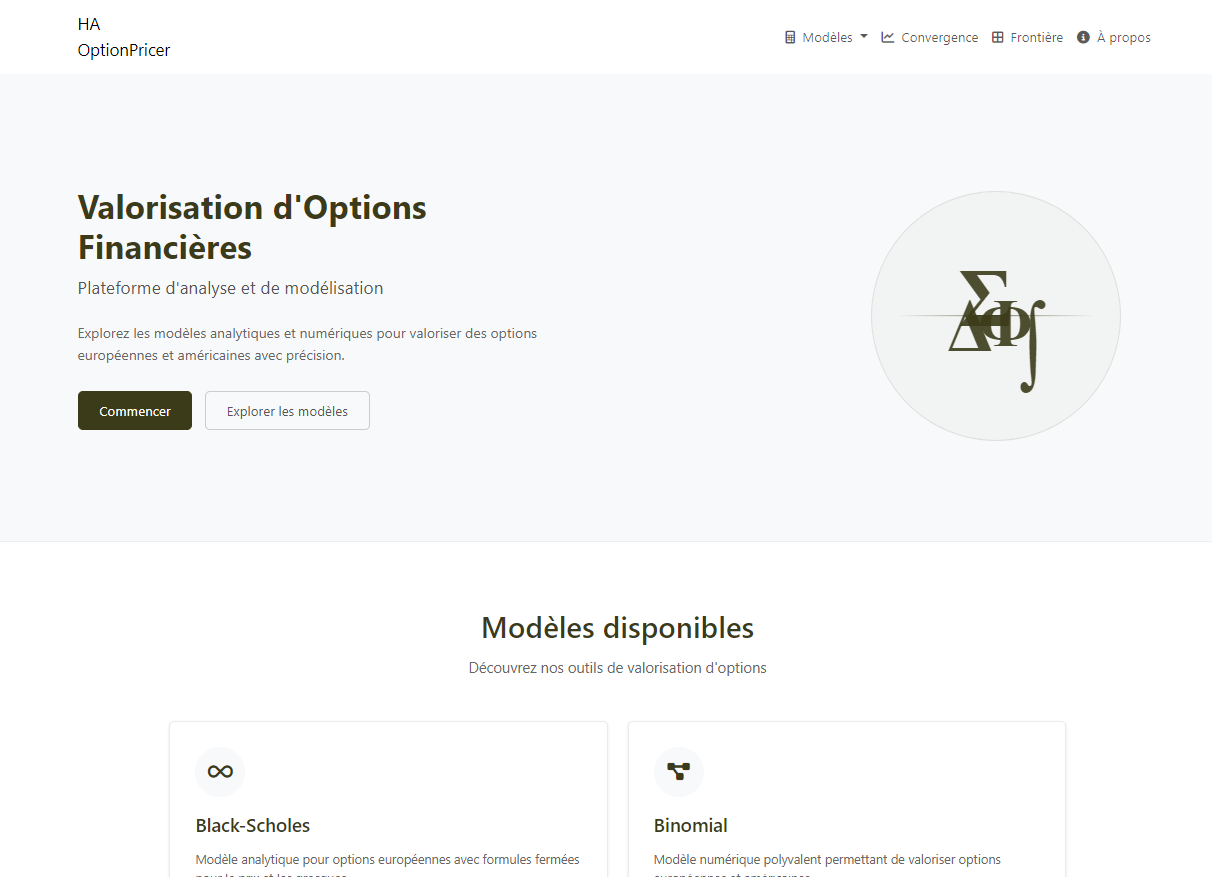
\includegraphics[width=0.9\textwidth]{images/acc1.png}
\caption{Page d'accueil de l'application OptionPricer}
\end{figure}
\begin{figure}[H]
\centering

\includegraphics[width=0.9\textwidth]{images/acc2.png}
\caption{Page d'accueil de l'application OptionPricer}
\end{figure}

L'application a été développée en utilisant Python (Flask) pour le backend et HTML/JavaScript pour le frontend. Les calculs financiers sont réalisés avec NumPy et SciPy, et les visualisations avec Plotly.js.

\section{Modèle Black-Scholes}

Le premier module de l'application permet de calculer le prix d'une option européenne selon le modèle de Black-Scholes ainsi que les grecques associées.

\begin{figure}[H]
\centering
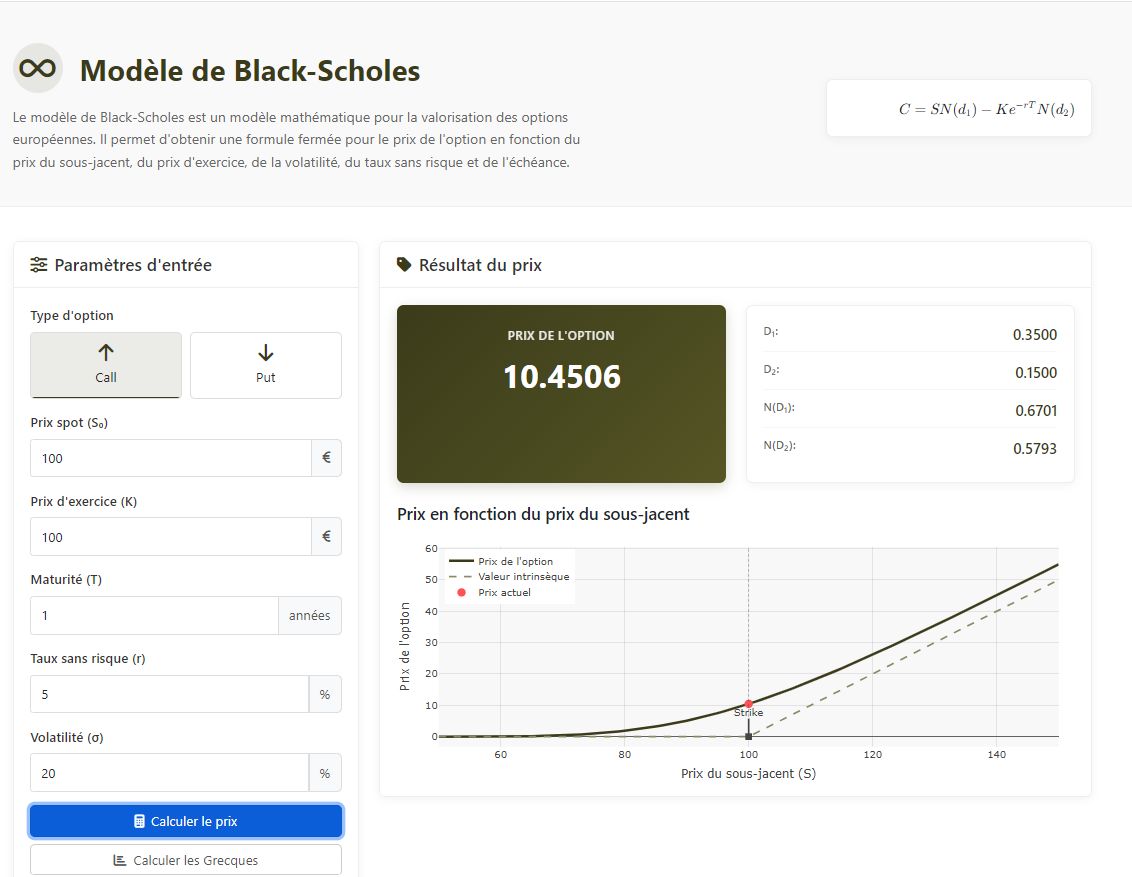
\includegraphics[width=0.9\textwidth]{images/BS1.png}
\caption{Module Black-Scholes avec calcul du prix et des grecques}
\end{figure}
\begin{figure}[H]
\centering
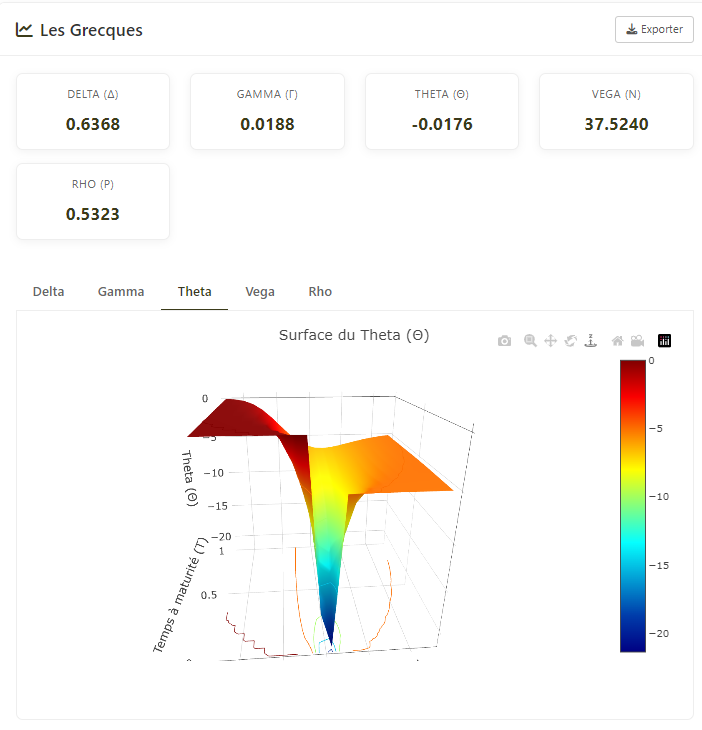
\includegraphics[width=0.7\textwidth]{images/GR.png}
\caption{calcul des grecques}
\end{figure}

L'utilisateur peut ajuster tous les paramètres (type d'option, prix spot, strike, maturité, taux et volatilité) et voir immédiatement l'impact sur le prix et les grecques.

\section{Modèle Binomial}

Le deuxième module implémente le modèle binomial, permettant de valoriser des options européennes et américaines.

\begin{figure}[H]
\centering
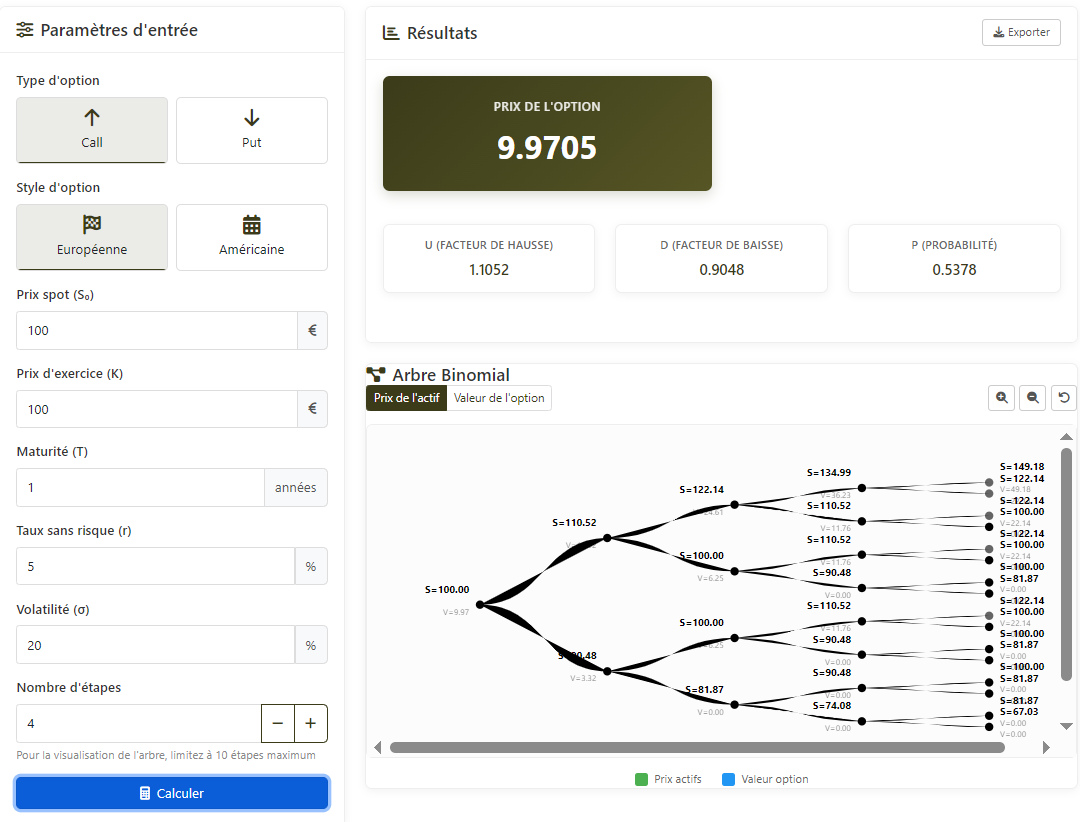
\includegraphics[width=0.9\textwidth]{images/BN.png}
\caption{Module du modèle binomial pour options européennes et américaines}
\end{figure}

L'application calcule le prix en temps réel et permet de comparer les résultats avec le modèle de Black-Scholes pour les options européennes.

\section{Analyse de Convergence}

Le module de convergence permet d'étudier comment le prix calculé par le modèle binomial converge vers celui de Black-Scholes lorsque le nombre d'étapes augmente.

\begin{figure}[H]
\centering
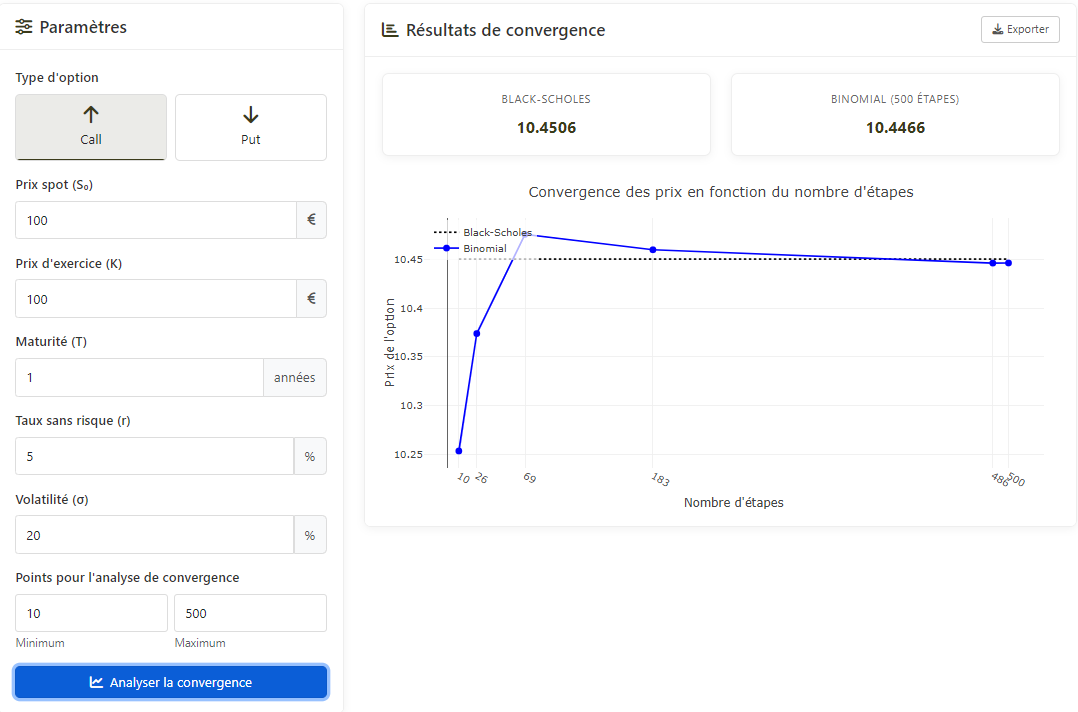
\includegraphics[width=0.9\textwidth]{images/Conv.png}
\caption{Analyse de convergence du modèle binomial vers Black-Scholes}
\end{figure}

Les graphiques montrent l'évolution du prix et de l'erreur en fonction du nombre d'étapes, illustrant la vitesse de convergence.

\section{Frontière d'Exercice Optimal}

Ce module constitue le cœur de notre application. Il calcule et visualise la frontière d'exercice optimal pour les options américaines.

\begin{figure}[H]
\centering
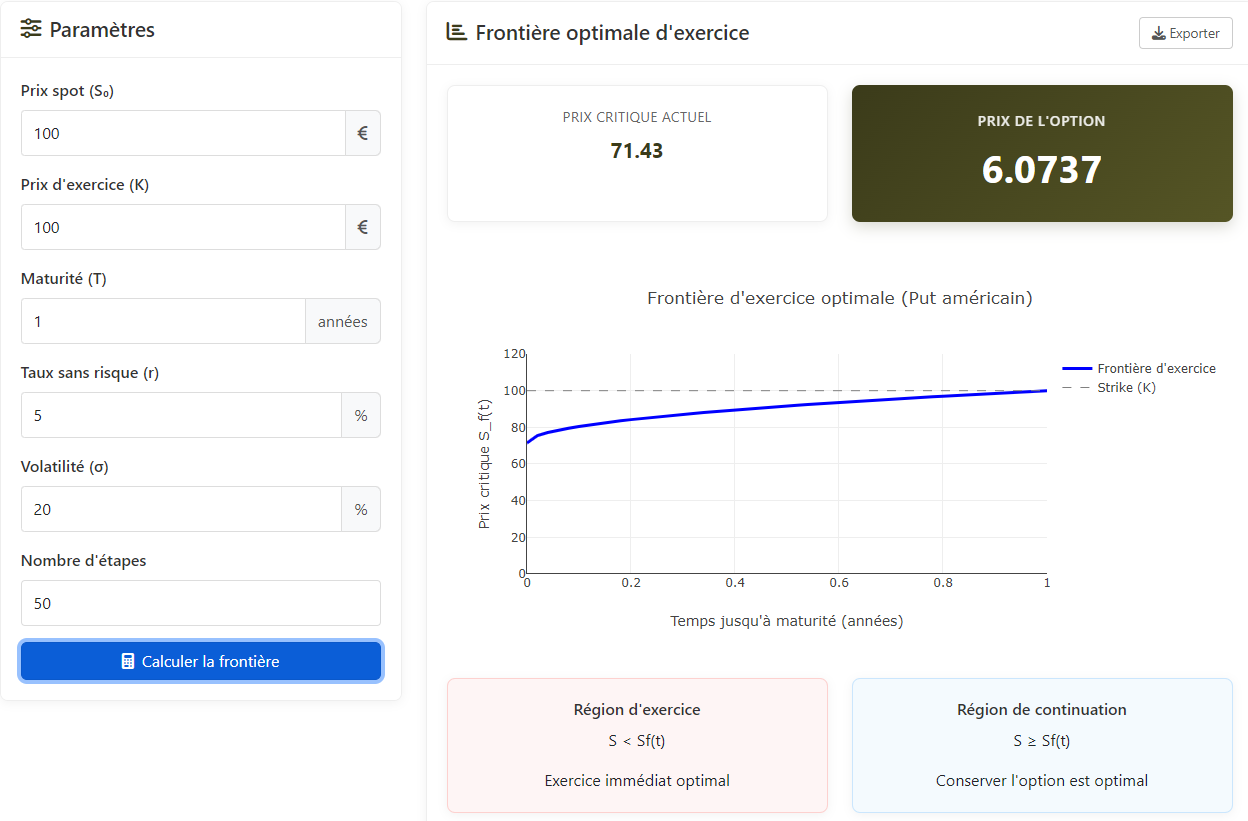
\includegraphics[width=0.9\textwidth]{images/FR.png}
\caption{Frontière d'exercice optimal pour un put américain}
\end{figure}

Le graphique montre comment la frontière d'exercice évolue au cours du temps, définissant clairement la région où l'exercice immédiat est optimal.

\section{Modèle à Régimes Markoviens}

La principale innovation de notre application est l'implémentation du modèle à régimes markoviens, qui permet d'étudier l'impact des changements de régime de volatilité sur la frontière d'exercice.

\begin{figure}[H]
\centering
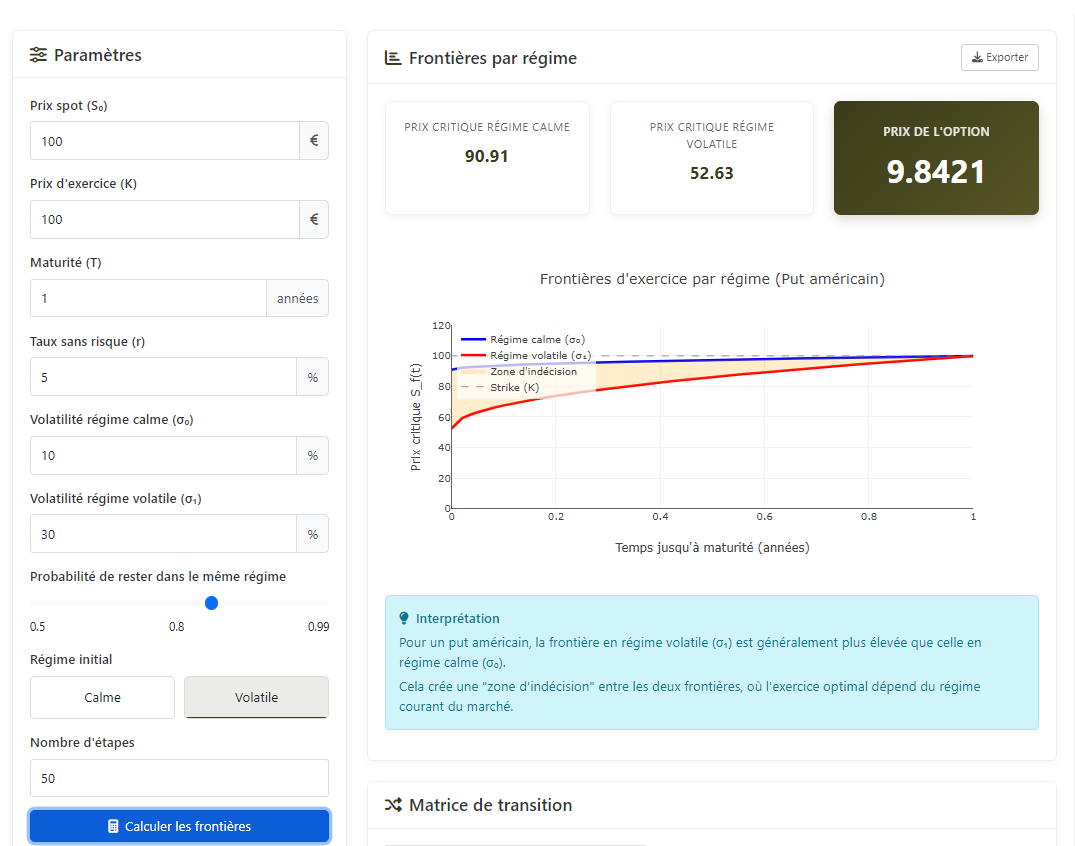
\includegraphics[width=0.9\textwidth]{images/Mark.png}
\caption{Frontières d'exercice optimal sous différents régimes de volatilité}
\end{figure}

Comme le montre la figure, le modèle calcule une frontière d'exercice distincte pour chaque régime (calme et volatile), faisant apparaître une "zone d'indécision" entre les deux.

\begin{figure}[H]
\centering
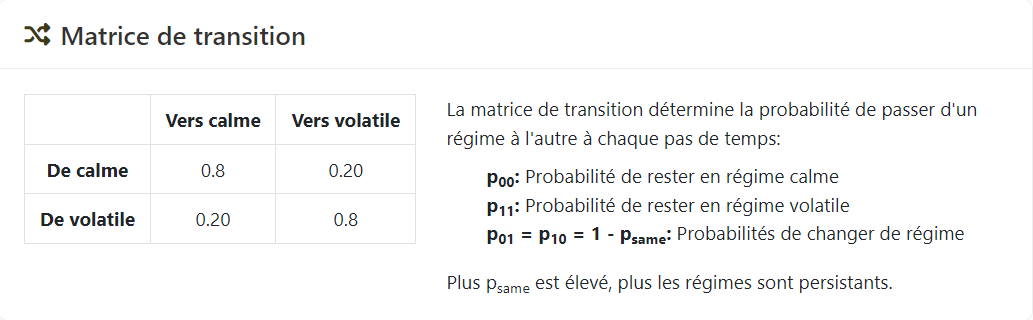
\includegraphics[width=0.9\textwidth]{images/MT.png}
\caption{Matrice de transition entre les régimes}
\end{figure}

L'application permet également de visualiser et d'ajuster la matrice de transition entre les régimes, illustrant comment les probabilités de transition affectent les décisions d'exercice.


\section{Conclusion et perspectives}

L'application OptionPricer offre un outil pratique et pédagogique pour l'étude des options américaines et de leurs frontières d'exercice optimal. L'intégration du modèle à régimes markoviens constitue une extension pertinente qui enrichit l'analyse des décisions d'exercice dans un contexte de marché plus réaliste.

Parmi les perspectives d'amélioration, on pourrait envisager:
\begin{itemize}
    \item L'intégration d'un module de calibration sur données réelles
    \item L'application à d'autres types d'options exotiques
\end{itemize}









\begin{thebibliography}{99}

\bibitem{CRR} Cox, J. C., Ross, S. A., \& Rubinstein, M. (1979). Option pricing: A simplified approach. \textit{Journal of Financial Economics}, 7(3), 229-263.

\bibitem{BS} Black, F., \& Scholes, M. (1973). The pricing of options and corporate liabilities. \textit{Journal of Political Economy}, 81(3), 637-654.

\bibitem{Hamilton} Hamilton, J. D. (1989). A new approach to the economic analysis of nonstationary time series and the business cycle. \textit{Econometrica}, 57(2), 357-384.

\bibitem{HullWhite} Hull, J., \& White, A. (1987). The pricing of options on assets with stochastic volatilities. \textit{The Journal of Finance}, 42(2), 281-300.

\bibitem{Longstaff} Longstaff, F. A., \& Schwartz, E. S. (2001). Valuing American options by simulation: a simple least-squares approach. \textit{The Review of Financial Studies}, 14(1), 113-147.

\end{thebibliography}




\end{document}